
\section{Introduction}
\label{sec:introduction-mcf10}


\begin{figure}
  \centering
  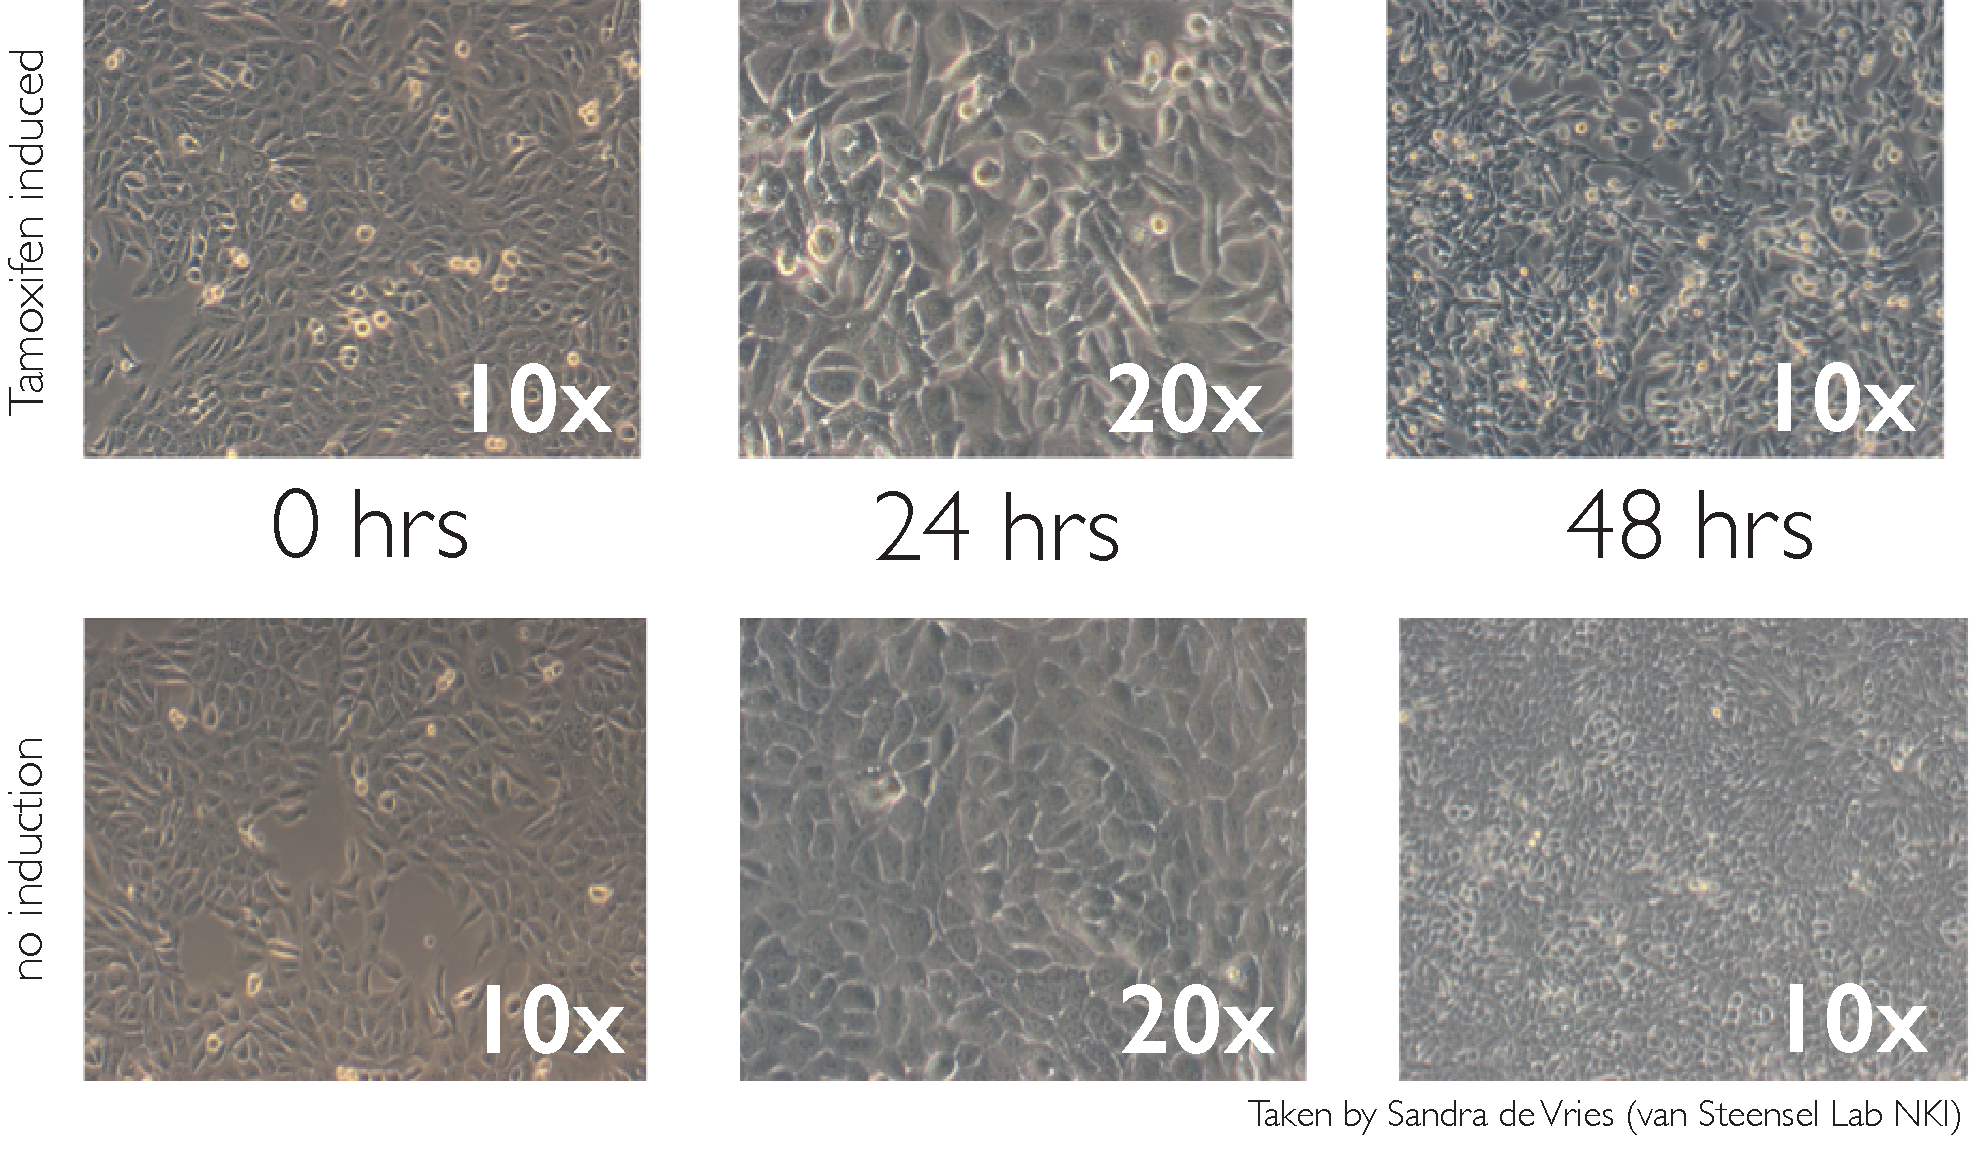
\includegraphics[width=1\textwidth]{pics/mcf10a-experiment}
  \caption{During the {\it in vitro} oncogenic transformation of an MCF10A-Er-Src cell line, morphological transformations can be observed between $24-36$ hours \citep{Hirsch:2010ec}. Here we show images taken of the experiment at three different time points. The initial measurement at $t=0$ hours and two subsequent measurements at $t=24$ and $t=48$ hours. The magnification level for each image is indicated in the figure. The top row shows images of the experiment where Src is induced by addition of Tamoxifen at $t=0$; the bottom row shows images taken at the same time points without addition of Tamoxifen. It is possible to see morphological changes at the final time point $t=48$ where after addition of Tamoxifen cells are elongated and overlapping compared to the tightly packed structure in the system without induction. These images were taken by Sandra de Vries in the van Steensel Lab at the NKI, Amsterdam}
  \label{fig:exp-pics}
\end{figure}

There are a variety of possible applications for the model outlined in Chapter \ref{cha:stamm}; examples include stem cell reprogramming \citep{Armond:2013} (contributions to which are discussed in Section \ref{cha:stem-cells}) and estrogen response of breast cancer cell lines \citep{Casale:2013}. Another example is oncogenic transformation which is the transition from healthy cells to cancer cells which we discuss in this Chapter. We consider a derivative of the human epithelial MCF10A cell line where the v-Src and estrogen receptor (ER) fusion is integrated; the new cell line is called MCF10A-Er-Src \citep{Hirsch:2010ec} (for brevity in the discussion that follows we will refere to these as MCF10A). The Src oncogene is activated by addition of tamoxifen resulting in a rapid transformation of this system. Morphological changes on a cellular level are observed as early as $t=24h$ (between $t=24h-36h$) they show the ability to form colonies in soft agar in the final transformed state \citep{Hirsch:2010ec} . Figure \ref{fig:exp-pics} shows images taken of one realisation of the experiment using a camera attached to a microscope; they are taken at $t= \lbrace 0, 24, 48 \rbrace$ hours at two different magnification levels ($10x$ and $20x$ as indicated on the figure). The top rows shows images taken after induction of tamoxifen and morphological changes in the cells can be observed. The bottom row shows a null where no tamoxifen is added and as expected we don't see any morphological changes just an increase in population density. A comparison between the final two images of the two sets is especially revealing as we can see cells elongated and overlapping cells in the induced system compared to tightly packed smaller cells.

In this Chapter we discuss one application of the two-step estimation pipeline of STAMM (see Section \ref{sec:estim-pipe}). We investigate the oncogenic transformation of an MCF10A cell line using  data obtained by performing RNA-seq measurements. This experiment was carried out for this work and the experimental design is summarised in Section \ref{sec:experimental-design}. In Section \ref{sec:norm-stand} we summarise the pre-processing step for RNA-seq measurements starting from integer count data to be used with STAMM. Then we present results from applying the estimation pipeline to RNA-seq data in Section \ref{sec:results-mcf10a}.

\section{Relevance}
\label{sec:relevance}

This is a very interesting system to consider mainly because it consists of only a single perturbation (i.e. induction of the classical oncogene v-Src) leading to tumorigenesis and as such is very clean. Additionally it is an exceptionally fast transformation (between $t=24-36$ hours) which makes repeat experiments to probe further properties of the systems or the verification of estimated parameters easy to implement. The transformation also leads to morphological changes which can be observed under a microscope. Moreover the initial state is a stable cell-line therefore tests or follow up experiments are easy to carry out.

\section{Experimental design}
\label{sec:experimental-design}

The data we analyse here was obtained by Sandra de Vries at the Netherlands Cancer Institue (NKI). The choice of time points was made considering the following criteria: to facilitate a better understanding of the system using results from previous work in \cite{Hirsch:2010ec}; to have sufficient data points to work well with STAMM; and the cost of each RNA-seq measurement. 
% uninduced: 0hr, 12hr, 24hr, 48hr
% For the second experiment I took along cells that were treated for 4 weeks with Plasmocin at 25ug/ml then cultured 2 weeks without Plasmocin and checked for mycoplasm with the Lonza mycoplasm detection kit. The cells tested negative but I found the morphology of the culture had changed, did not the nice cobblestone like morphology as before.
% I took in culture this batch of cells and the previous mycoplasma containing batch of cells and redid the experiment on a smaller scale
% Now of both I took the following timepoints as before and sent them to the microarray facility
% t= 0hr, 20hr and 48hr

The experiments were performed in MCF10A-Er-Src cells, a derivative of mammary epithelial cell line MCF10A containing an integrated fusion of the v-Src oncoprotein with the ligand binding domain of ER \citep{Hirsch:2010ec,Iliopoulos:2009do}. The cells were cultured in DMEM/F12 medium supplemented as described in \cite{Debnath:2003km}. There are two starting points and for both the medium is refreshed, then a medium containing $1 \mu M$ activating tamoxifen is added and the mixture is grown to a $80 - 85\%$ confluency population, and induced and uninduced samples were harvested at the time points $ 0h$, $ 0.5h$, $ 1h$, $ 2h$, $ 4h$, $ 6h$, $ 8h$, $ 10h$, $ 12h$, $ 24h$, $ 28h$, $ 32h \text{ and } 48h$ for RNA isolation. The second series is started when the first one is at $8h$ and samples collected at $0h$, $2h$, $4h$, $16h$, $18h$, $20h$, $24h$, and $40h$. Time points are collected as follows: wash with PBS; add 2ml Trizol resuspend thoroughly and store at $-80^{\circ}C$. The tamoxifen stock was made by dissolving 5mg in 12.9ml $96\% EtOH = 1mM$ stock. We did not send all the samples to the microarray facility, only the following (due to cost considerations): 

\textbf{1st series}: $0h$, $0.5h$, $1h$, $2h$, $4h$, $6h$, $8h$, $12h$, $16h$, $20h$ and $24h$

\textbf{2nd series}: $0h$, $24h$, $32h$, $40h$ and $48h$ \\
The RNA was isolated by the Trizol method, and prepared for sequencing by the Illumina RNA TruSeq sample protocol.


\section{Pre-processing data}
\label{sec:norm-stand}

As described in Section \ref{sec:rna-sequencing}, RNAseq data obtained from samples results in integer counts for genes corresponding to the number of times a sequenced strip belongs to a particular gene. To ensure that we are able to compare samples from different experiments in different setting the first step is to \emph{normalise}. Many methods exist to normalise sequencing experiments. We pre-process the data using the \texttt{edgeR} package in R \citep{McCarthy:2012wg,Robinson:2010cw}. One important assumption is that most genes are not differentially expressed between samples. To determine genes that are not differentially expressed the procedure uses a robust estimate for the ratio of RNA between samples: the weighted trimmed mean of M values (TMM). Two parameters are employed to filter out genes that are differentially expressed; the M-values, log-fold-changes, and the A-value, absolute expression levels. The cut-off set for both the M-value and the A-value is tuneable and the best way to set the tuning parameters is to select a range of cut-off parameters and determine when they stabilise (see Appendix \ref{sec:sequencing-depth-rna}). It is important to remember \texttt{edgeR} was developed to analyse differential expression \citep{Robinson:2010dd}, still the assumptions are also applicable to time course such as the data set for the oncogenic transformation. Note without this step it is not possible to compare data from different samples.

After the first pre-processing step we still can't use the data in our model because the likelihood is based on an additive Gaussian noise model (eqn. (\ref{eq:likelihood})). For RNA-seq data once it has been \emph{normalised} the next pre-processing step is to transform the data such that distorting effects at high expression values are reduced. We use a nonlinear transform proposed by \cite{Hoffman:2012gn} the $\arcsinh x = \ln(x + \sqrt (x^2 + 1))$. The advantage of using this transformation compared to the more regularly used $\ln x$ is that it has the same effect of reducing variance at higher values but a much smaller effect at lower values. Now after applying these two pre-processing steps we can use this data in our model.

\section{Results}
\label{sec:results-mcf10a}

\begin{figure}
  \centering
  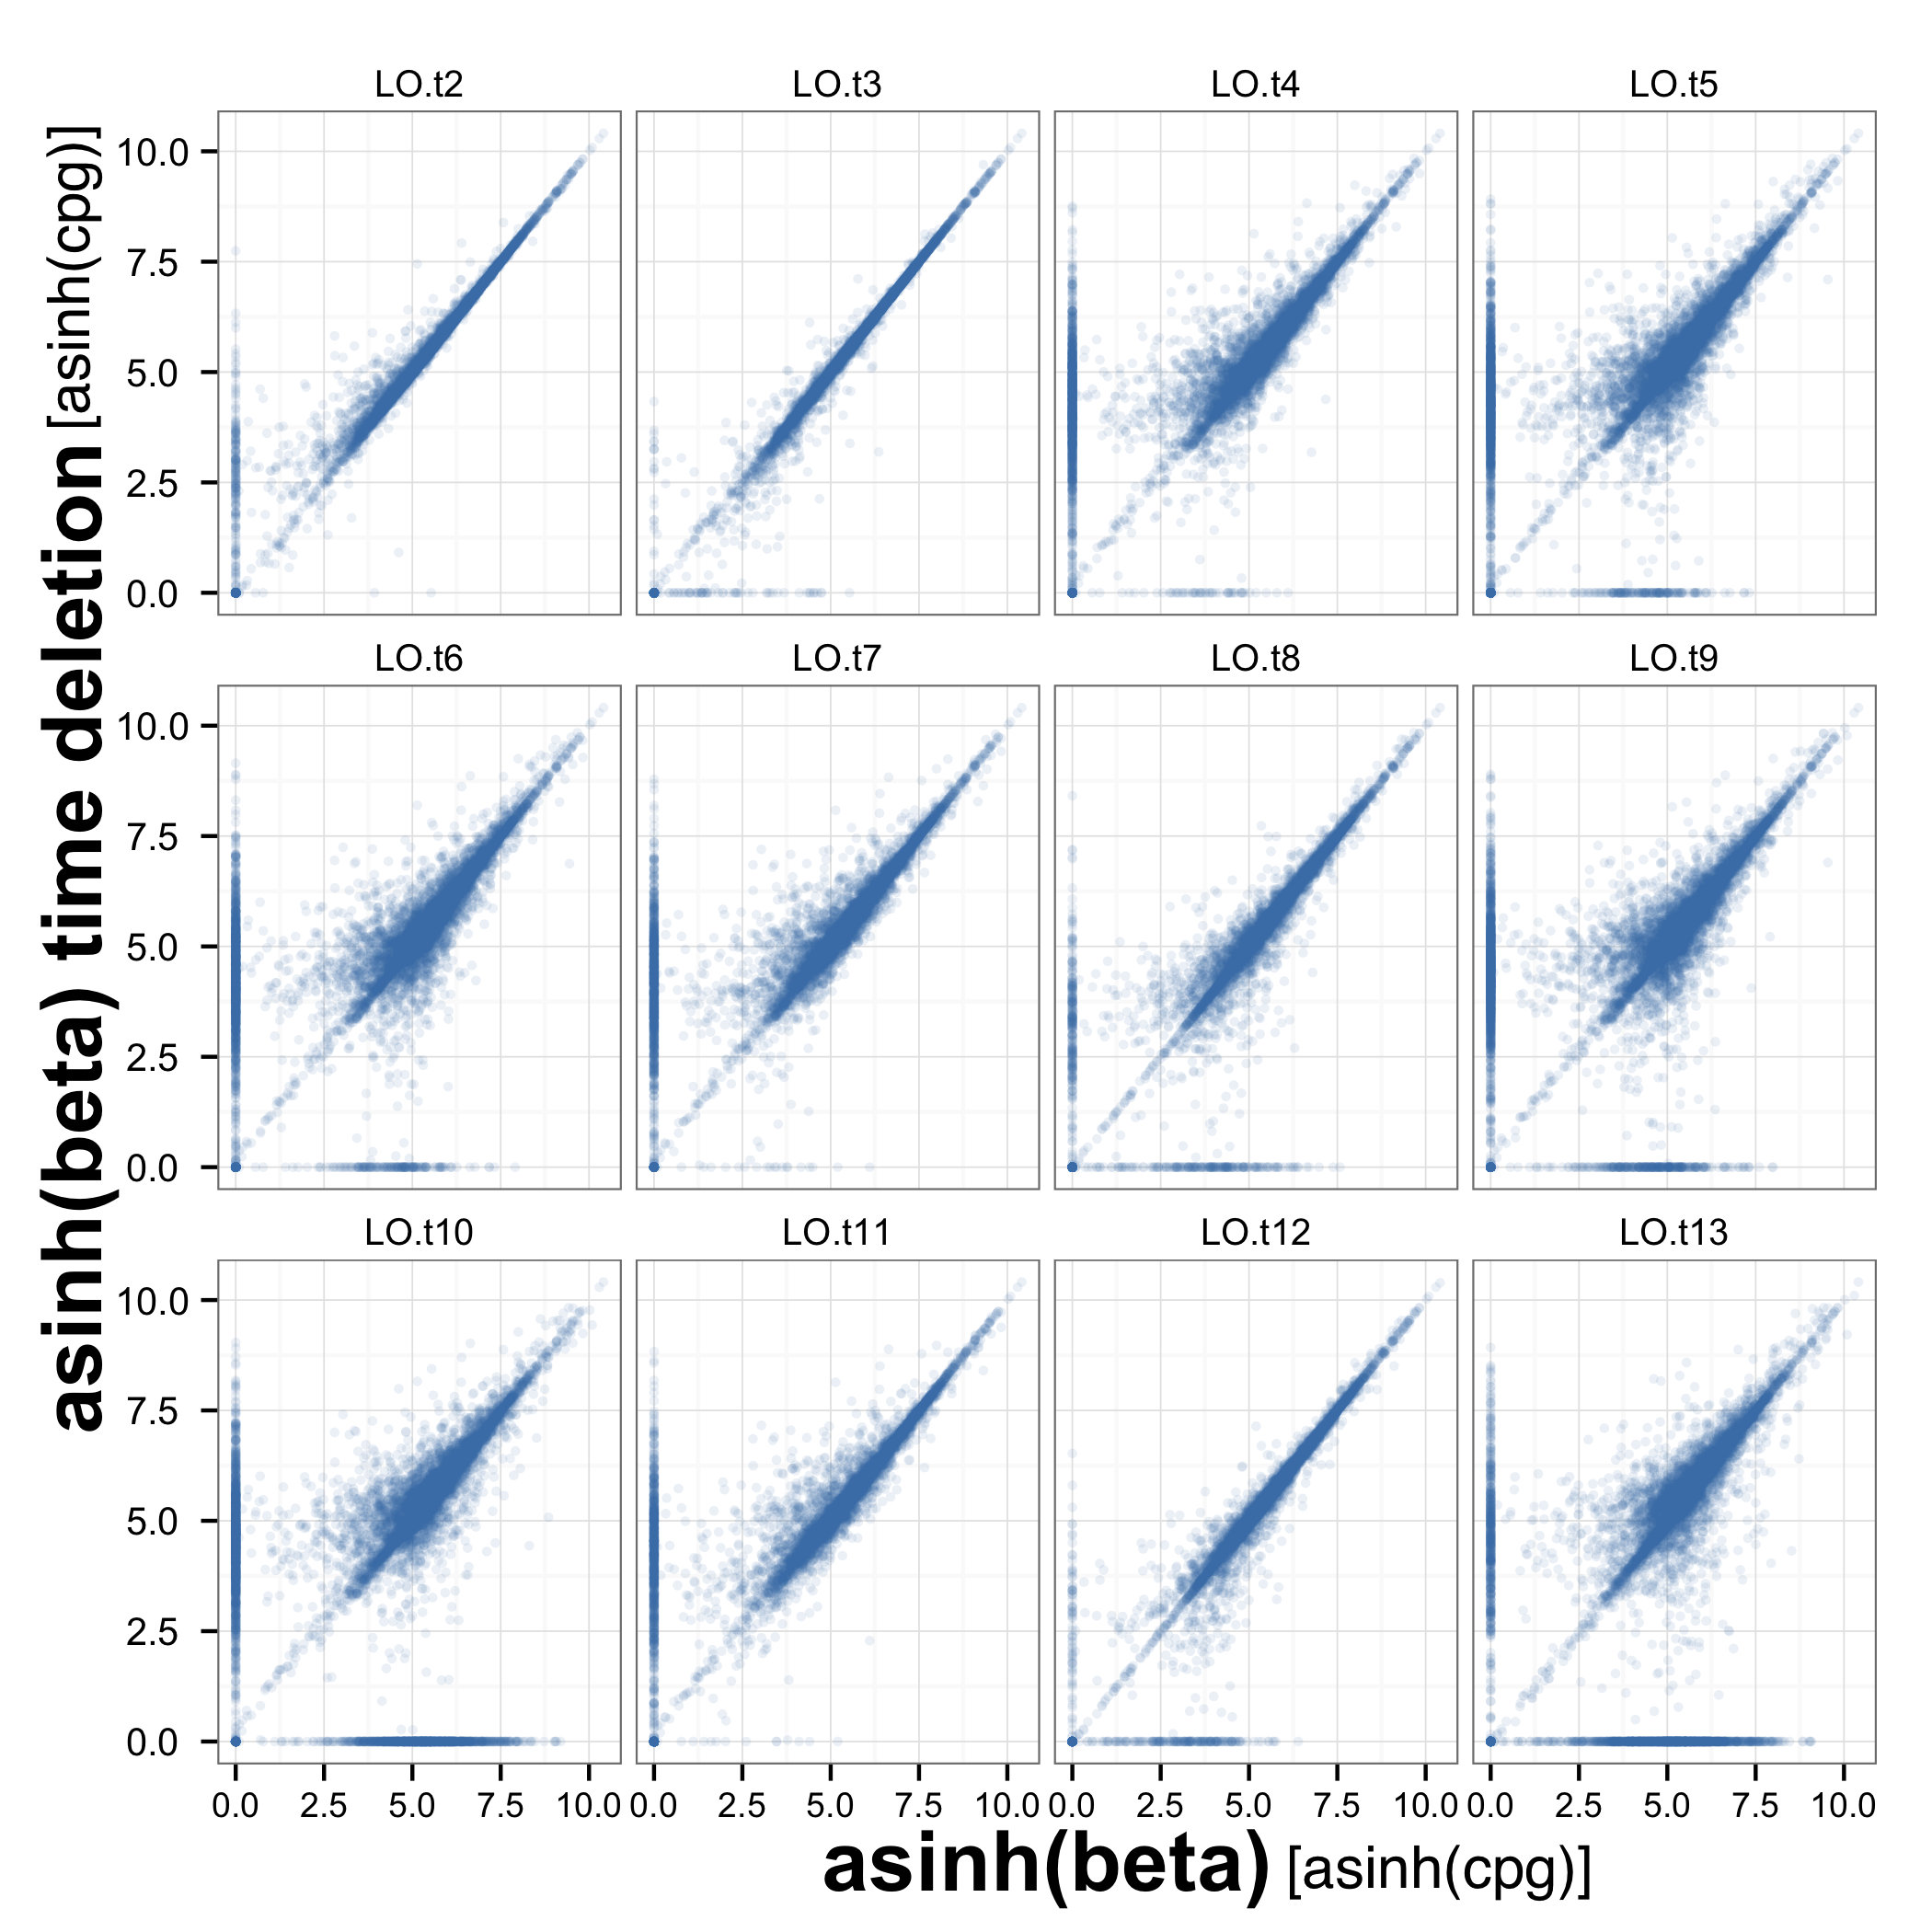
\includegraphics[width=0.9\textwidth]{pics/no-pen-data.png}
  \caption{The RNA-seq measurements are filtered with respect to standard deviation (we filter out genes with $\sigma_j > 20$ before transformation) because we are interested in genes that change significantly in time. This plot scatters estimated expression signatures using all time points to estimates where one time point is dropped. This tests stability of estimates to determine need for $\ell_1$ penalisation under deletion of time points. The estimates are stable (Pearson correlations is $>0.8$ therefore we conclude that there is no need for a penalty term.}
  \label{fig:data-pen}
\end{figure}

\begin{figure}
  \centering
  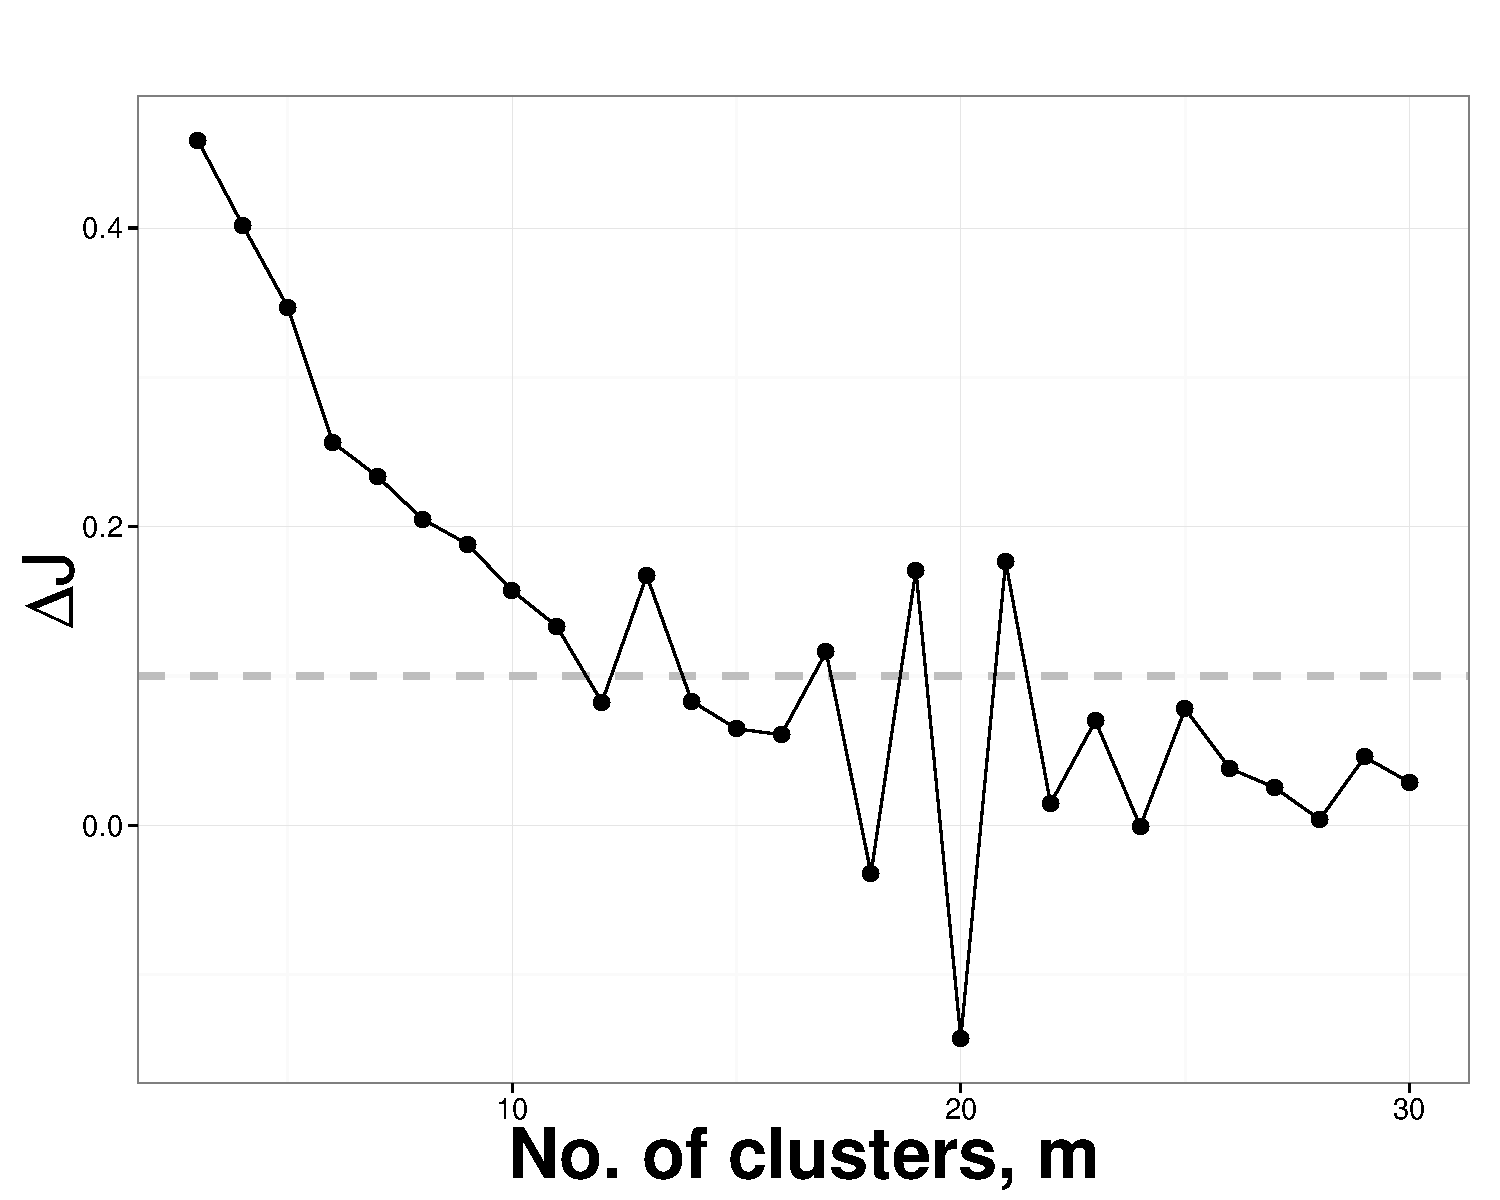
\includegraphics[width=0.7\textwidth]{pics/kmeans-dat.pdf}
  \caption{K-means clustering of {\it in vitro} data for the transformation of an MCF10A cell line. Initial k-means clustering is performed to identify representative trajectories. As described in Section \ref{sec:estim-pipe} we choose the optimal number of clusters $\hat{m}$ by considering relative changes in the objective function $\Delta J (m) = (J(m-1) - J(m))/J(m-1)$; we set $m$ where $\Delta J(m-1) < 0.1$. The plot shows $\Delta J$ as a function of $m$ and the horizontal dashed line represents our threshold at $0.1$. For this example we can see that the $\hat{m} = 13$. Note that fluctuation in $\Delta J$ at higher $m$ are due to small values of $J(m)$. }
  \label{fig:kmeans-dat}
\end{figure}

The data obtained uses RNA-seq to examine changes in gene expression during this transformation time-course with $T=13$ time points\footnote{$t=\lbrace 0, 0.5,  2,  4,  6,  8, 12, 16, 20, 24, 32, 40, 48h \rbrace$, at $t=0$ and $t=20$ we have a repeated measurements}. According to the assumption in our model all cells are in the initial state at $t=0$. Here, by experimental design, the initial state consists of the derivative MCF-10A-Er-Src cell line fulfilling this assumption. More specifically the time point $t=0$ corresponds to the initial treatment with Tamoxifen an anti-oestrogen drug that binds to ER activating v-Src. Of course this is only the case excluding any unidentified epigenetic heterogeneity in the initial cell culture.  Therefore it is reasonable to assume that the cell population is approximately homogenous and comprised mainly of untransformed MCF-10A cells.



\begin{figure}
  \centering
  \subfigure[Number of state $K$]{
    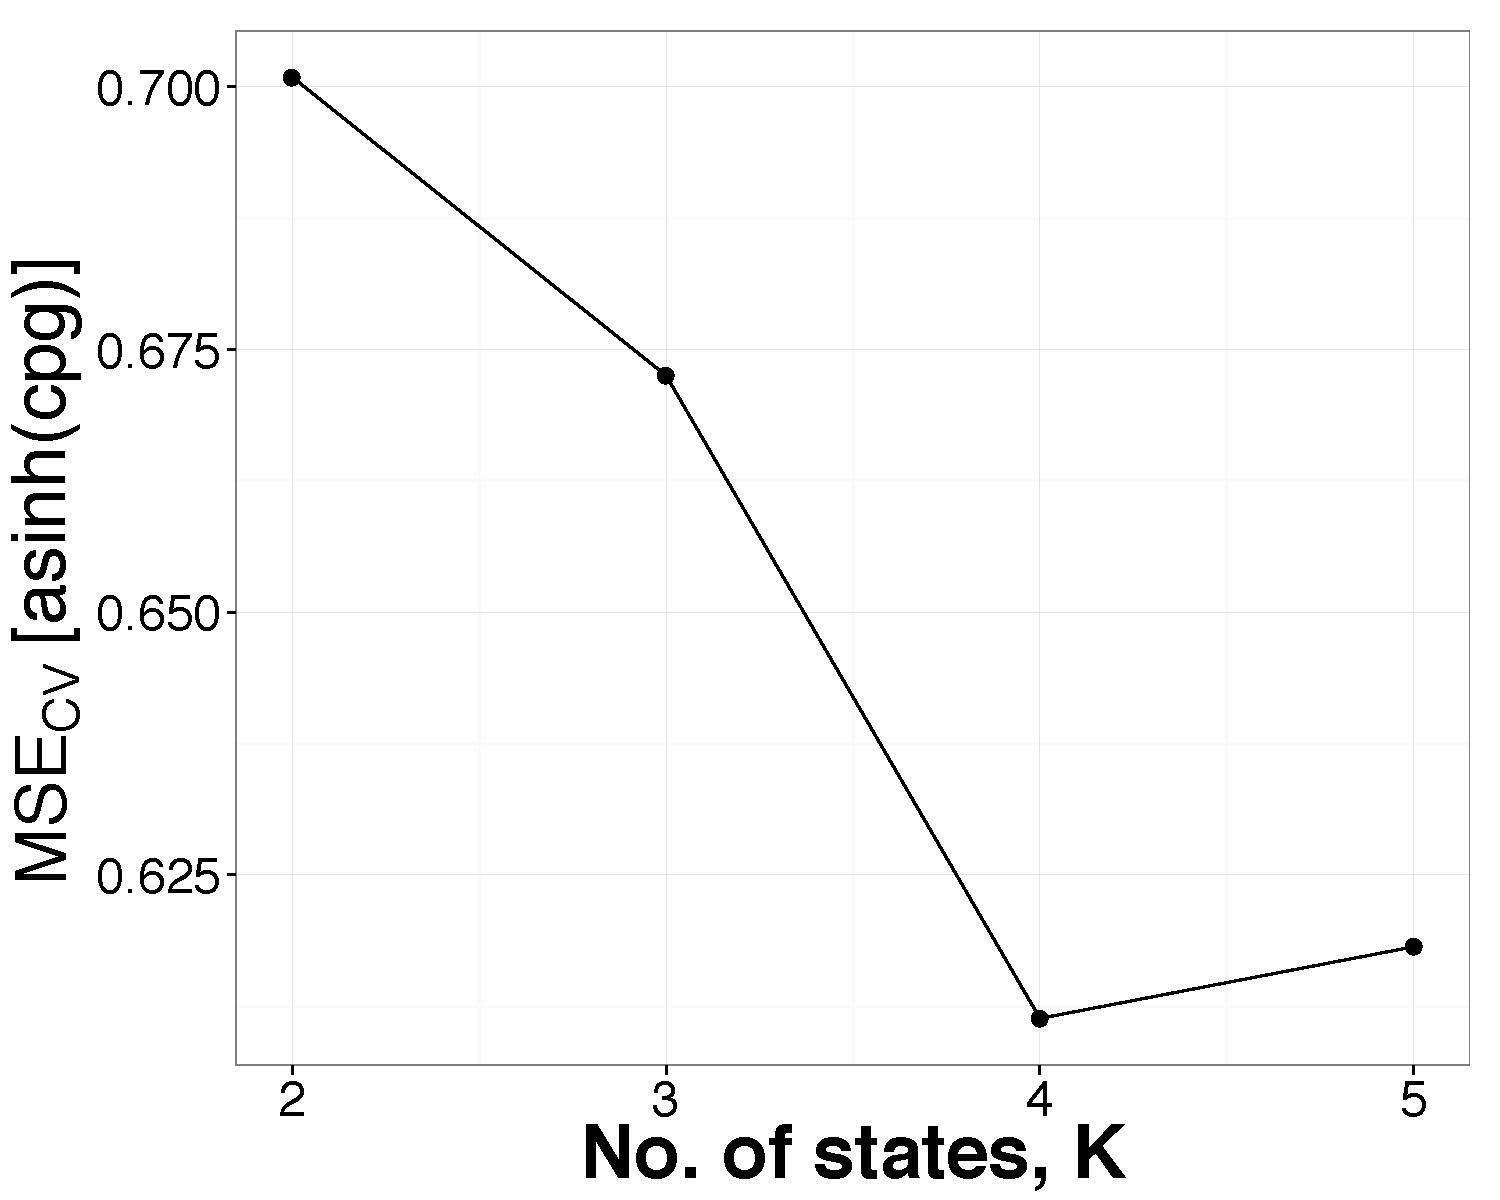
\includegraphics[width=0.45\textwidth]{pics/loocv-dat.pdf}
    \label{fig:data-m}
  }
  \subfigure[Stability of number of cluster]{
    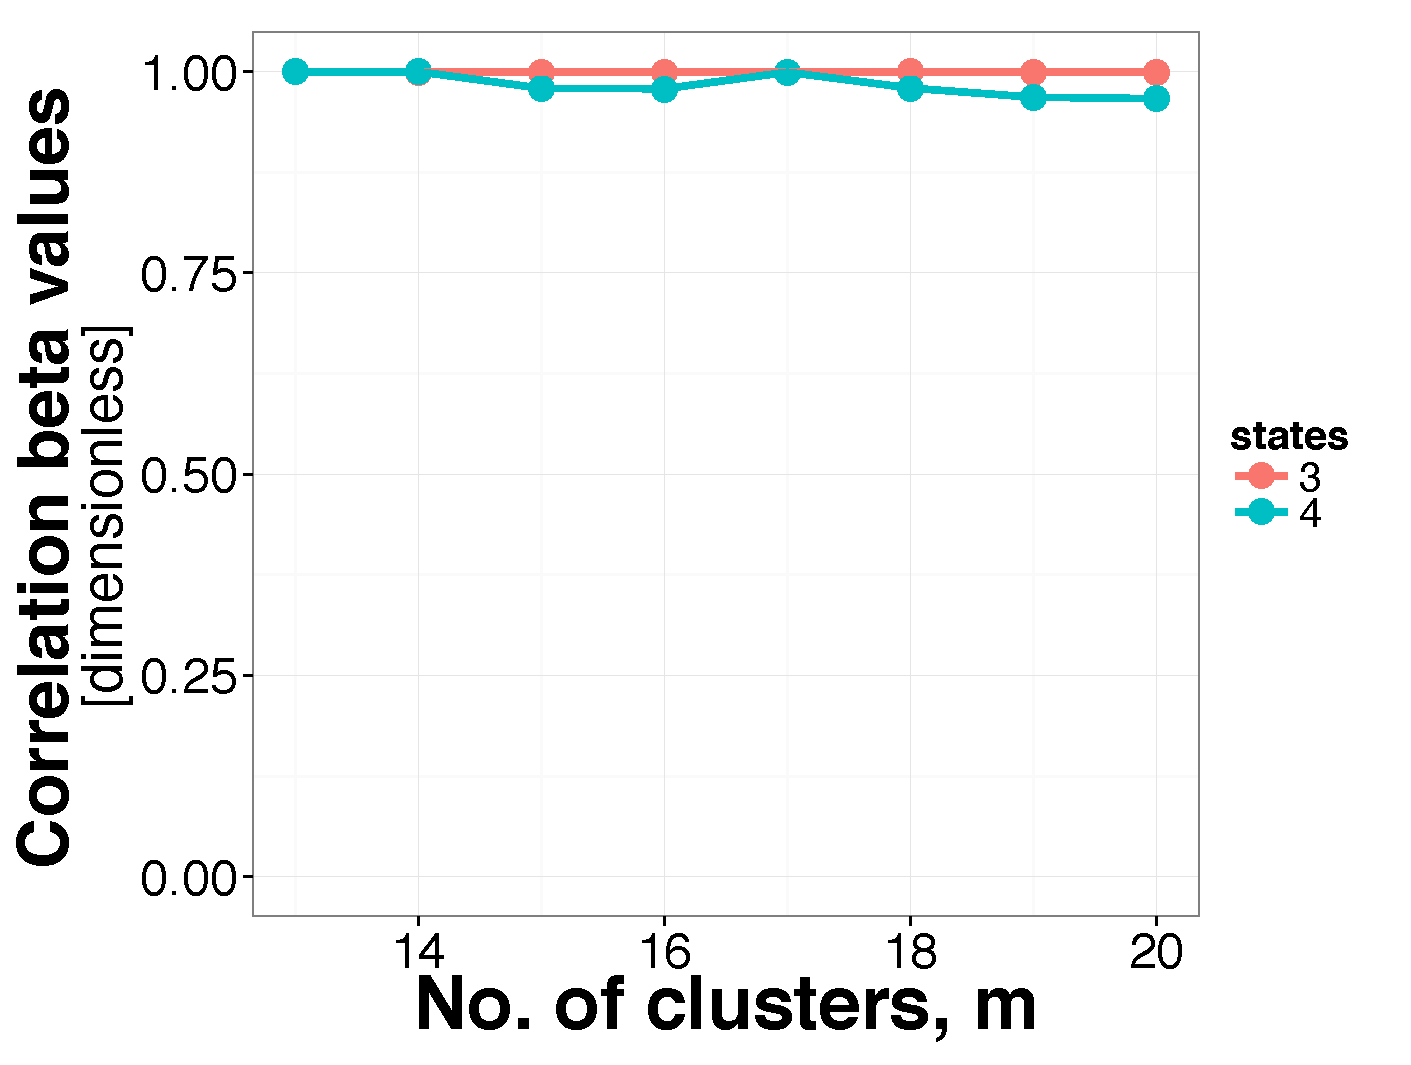
\includegraphics[width=0.45\textwidth]{pics/stab-m-dat.pdf}
    \label{fig:data-stab-m}
  }
    \caption{MCF-10A data. \subref{fig:data-m} $\mathrm{MSE_{CV}}$ score as a function of $K$. The minimum at $K = 4$ shows the optimal number of states for this oncogenic transformation. \subref{fig:data-stab-m} To determine if the choice of $\hat{m}$ in the k-means clustering algorithm was chosen correctly a stability test is performed. Correlations are calculated between expression signatures estimated between the $\hat{m}$ used and larger $m$. Here we find the clustering is close to one for $K=3$ and $K=4$ therefore the choice is reasonable.}
  \label{fig:data-m-k}
\end{figure}

\begin{figure}
  \centering
  \subfigure[Gene trajectories]{
    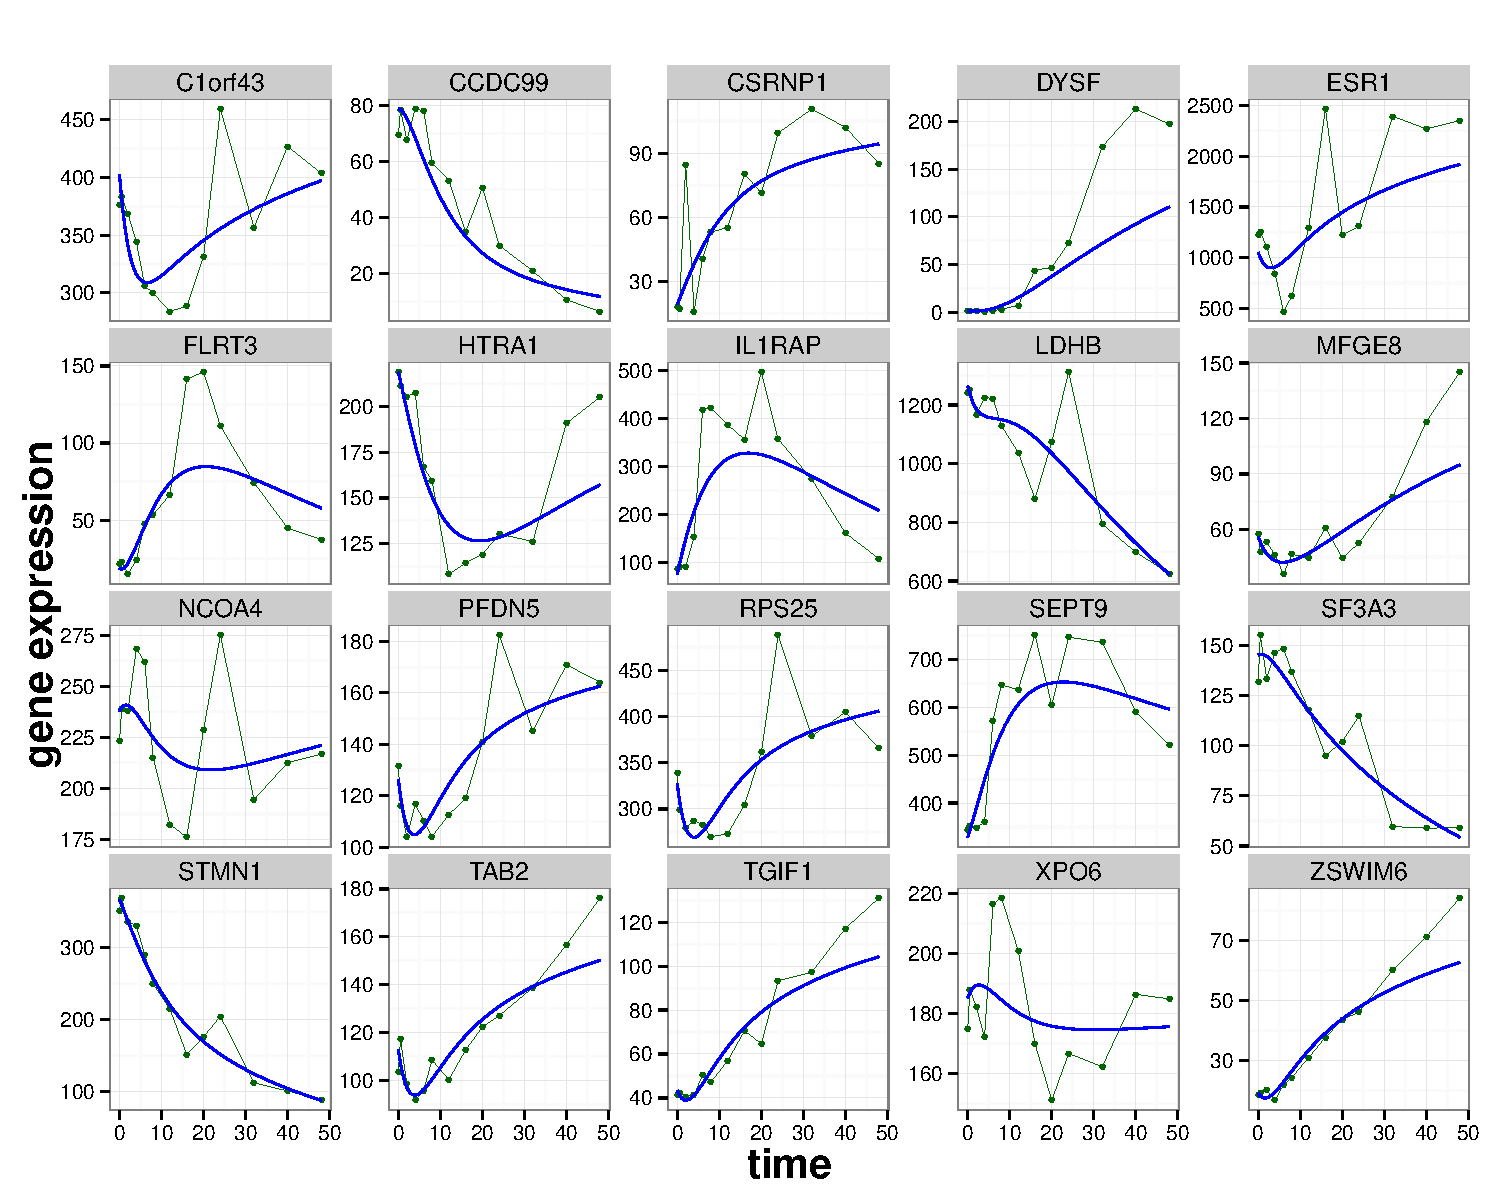
\includegraphics[width=0.75\textwidth]{pics/traj-dat1.pdf}
    \label{fig:data-traj}
  }
  \subfigure[Expression signatures]{
    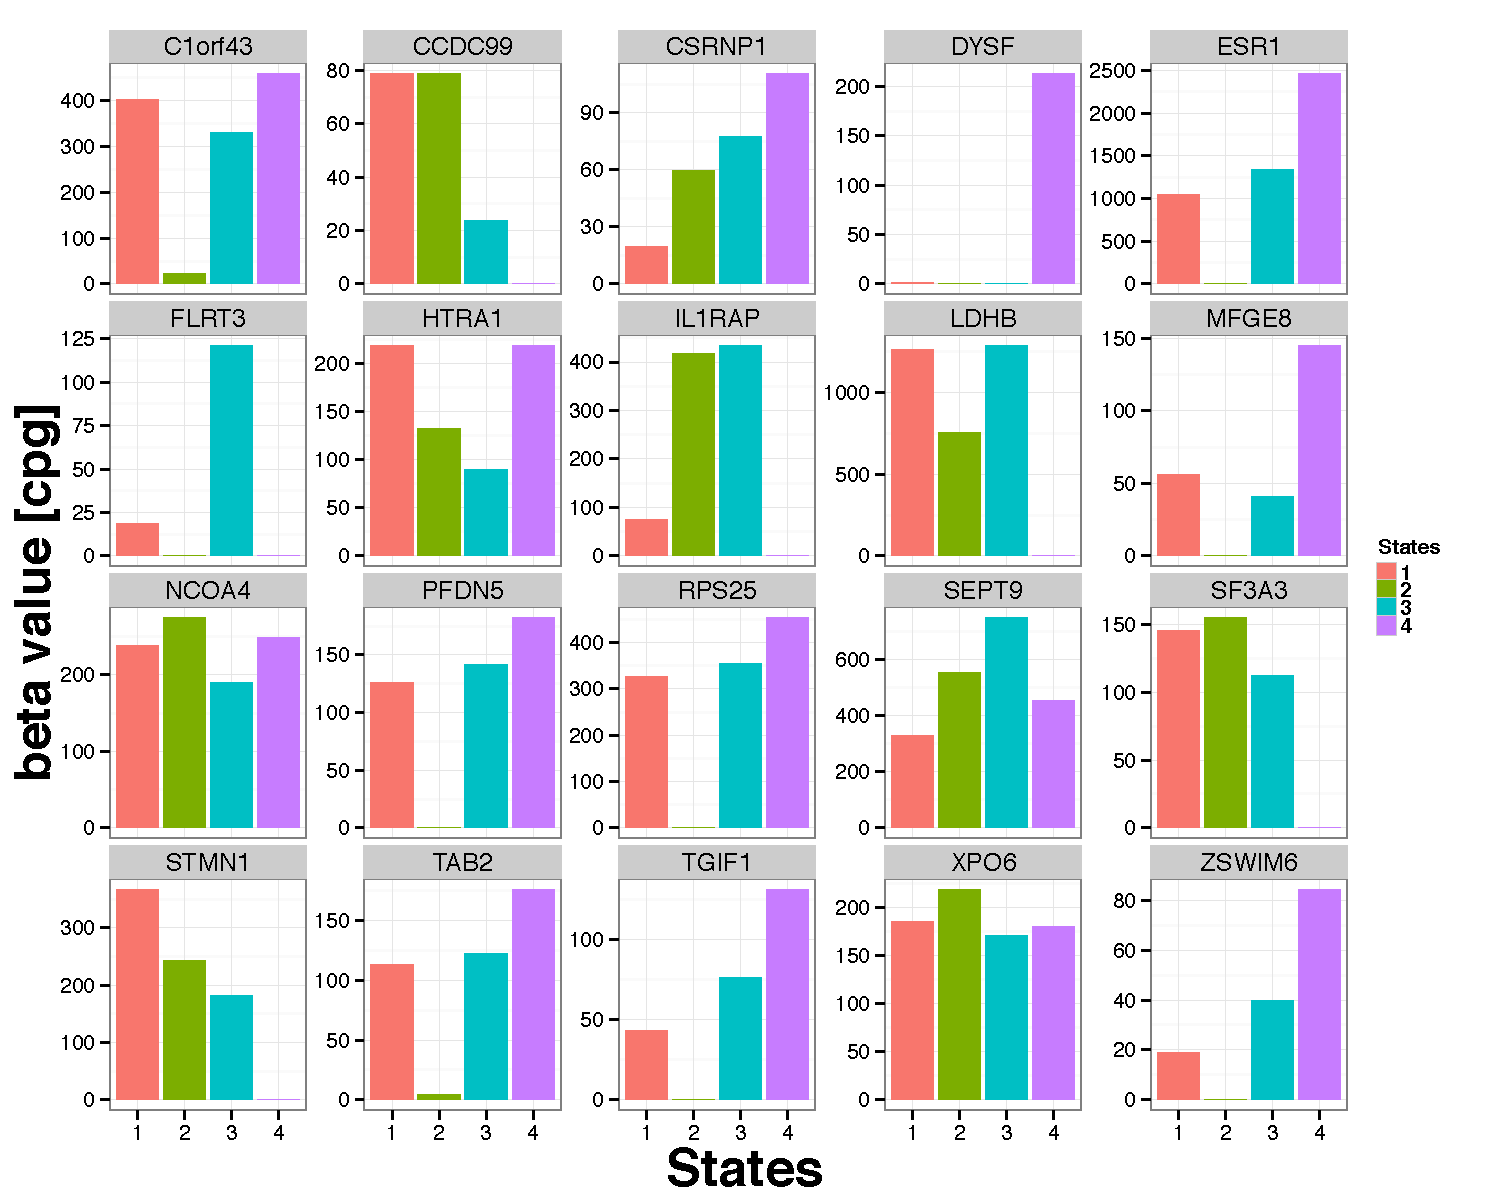
\includegraphics[width=0.8\textwidth]{pics/traj-dat2.pdf}
    \label{fig:data-beta}
  }
  \caption{MCF-10A data. \subref{fig:data-traj} The green line connects data points from measurements on the oncogenic transformation of MCF-10A cell-line. The blue line shows predicted trajectories from the model using estimated parameters. We can see that the model fits the trajectories well. \subref{fig:data-beta} The estimated $\beta_{kj}$ values for the trajectories are plotted here as bar charts. We can see that there are diverse expression signatures present in the data.}
  \label{fig:data-fit-traj}
\end{figure}

We want to focus our investigation only on genes that change during the experiment. To that end we filter out all genes $j$ where the standard deviation $\sigma_j$ is too small, setting the threshold at $\sigma_j > 20$ (on the linear scale, over time). This still leaves $p=2809$ gene expression trajectories to which we apply STAMM. We carried out parameter estimation as described in Section \ref{sec:estim-pipe} using a two-step process. The initial step is to perform a stability test, determining the need for a penalty term by comparing estimated expression signatures from the whole data set and data sets with left out time points. We conclude from the results in Figure \ref{fig:data-pen} that there is no need for a penalisation. The next step is to cluster the data using k-means clustering where we want to use cluster centroids to estimate transition rates for the next step. We conclude from Figure \ref{fig:kmeans-dat} that the optimal number of cluster  $\hat{m}$ is $13$. We use this result to perform model selection using cross-validation for $k=\lbrace 1, \ldots, 5\rbrace$. We find that the $\mathrm{MSE_{CV}}$ score shows a minimum at $K=4$ states (see Figure \ref{fig:data-m}). This would suggest two distinct intermediate states in the oncogenic transformation of MCF-10A cells. Figure \ref{fig:data-traj} shows a representative set of trajectories from RNA-seq data in green and the blue lines shows predicted trajectories using estimated parameters. Overall we find that the model performed well and fits even diverse trajectories well. State-specific gene expression signatures corresponding to these trajectories are shown in Figure \ref{fig:data-beta}. These values show distinct patterns that would allow for filtering out surface markers distinguishing states. The final step of the estimation pipeline is to check sensitivity of estimation due to an increase in the number of clusters $m$. This test is performed by computing correlation between expression signatures estimated using $\hat{m}$ clusters and higher numbers of clusters. Figure \ref{fig:data-stab-m} shows the correlations as a function of $m$ for $K=3$ and $K=4$ and we find that the estimates are stable and therefore $\hat{m}$ was chosen well.

This concludes the application of STAMM to the RNA-seq time course for an oncogenic transformation. The example illustrates the application of the model to novel RNA-seq data can be carried out efficiently. However to investigate and validate of the intermediate states further experiments are needed since the current time-course is biologically not viable for further study (see discussion below) this has to be left as future work. 

\section{Discussion}
\label{sec:discussion-onco}

We applied the estimation pipeline (see Section \ref{sec:estim-pipe}) to time course data obtained by {\it in vitro} experiments for oncogenic transformation of a MCF-10A cell line. The systems has many fascinating properties, the fact that it undergoes a rapid state transition between phenotypically distinct states makes it a very useful system to study. Even though the driver for the transformation is one of the most well studied oncogenes there are still many open questions about epigenetic and genetic changes  during this process as well as general oncogenic transformations. Note that due to a mycoplasm infection in  the cells used for the {\it in vitro} study substantive  biological conclusions can be drawn only with extreme caution. Additional experiments are needed to verify the validity of the time-course data first. 

This application serves only the purpose of illustrating that STAMM can be applied to RNA-seq data yielding useful results. Though in future due to the clean and relatively rapid transformation in the system it is very useful to validate some claims from the model. It would also serve well as an example system to extend the model to include verification steps after an initial application followed by application of a more detailed model. If it is possible to find surface markers that allow us to distinguish specific states it should also be possible to get more detailed information on the latent process i.e. measure transition rates between states and maybe include backward transition to obtain more precise estimates for state-specific expression signatures.


Model selection for $k = \lbrace 2 \ldots 5 \rbrace$ and estimation for all parameters for the RNA-seq dataset was performed after applying threshold on the expression count leaving us with $p=2809$ genes. Computation took $3.8$ hours on 50 cores each with an AMD $2600MHz$ cpu. 



%%% Local Variables:
%%% TeX-master: "warwickthesis"
%%% End:
